\section{Introducci�n}
% v5.0: corregida por el tribunal.
Debido a la creciente disponibilidad de las plataformas m�viles y el gran poder de procesamiento con el que cuentan, el n�mero de aplicaciones m�viles ha crecido de manera significativa en los �ltimos a\~nos. Dichas plataformas cuentan con sistemas de adquisici�n de audio, video y una variedad de sensores como por ejemplo aceler�metro y giroscopio, lo que las transforma en sistemas ideales para desarrollar aplicaciones de procesamiento multimedia.\\
Por otro lado, desde hace algunos a\~nos varios museos de distintas partes del mundo han comenzado a considerar este tipo de dispositivos, y otras tantas tecnolog�as, como una alternativa muy interesante para brindar un valor agregado al usuario. Proyecciones de im�genes y videos, recorridos interactivos y aplicaciones de \textit{realidad aumentada} son tan s\'olo algunos de los ejemplos. Sin embargo, esta es un �rea muy reciente y en la que todav�a queda un camino muy largo por recorrer.\\
Durante el proyecto de fin de carrera se desarroll� sobre dispositivos m�viles un recorrido interactivo para un museo, con realidad aumentada. Probablemente, la realidad aumentada sea el mayor atractivo del proyecto por ser un �rea que se encuentra en pleno desarrollo y que todo el tiempo recibe ideas innovadoras y muy interesantes, lo que la hace por dem�s apasionante. Vale la pena entonces dar una definici�n para la misma:\\

\textit{La realidad aumentada (AR del ingl�s \textit{Augmented Reality}) es un t�rmino que denota la visi�n de un entorno f�sico del mundo real, cuyos elementos se combinan con elementos virtuales generados por computadora, para la creaci�n de una realidad mixta en tiempo real.}\\

Cuando se genera una imagen por medio de realidad aumentada, conviven en ella elementos reales con elementos virtuales. Es b�sicamente un juego de percepciones. En la Figura \ref{fig: arIntro} se muestra un ejemplo de realidad aumentada desarrollado durante este proyecto. Se puede ver en ella, un cubo virtual sobre la esquina superior izquierda de ``Hombre de Vitruvio'' de Leonardo da Vinci, de manera coherente con la posici�n del dispositivo respecto de la obra. Si en esta figura tan s�lo se viera a trav�s del dispositivo, cualquiera podr�a pensar que el cubo es real y que efectivamente forma parte de la escena. Eso es lo que busca la realidad aumentada. \\
\begin{figure}[H]
        \centering
        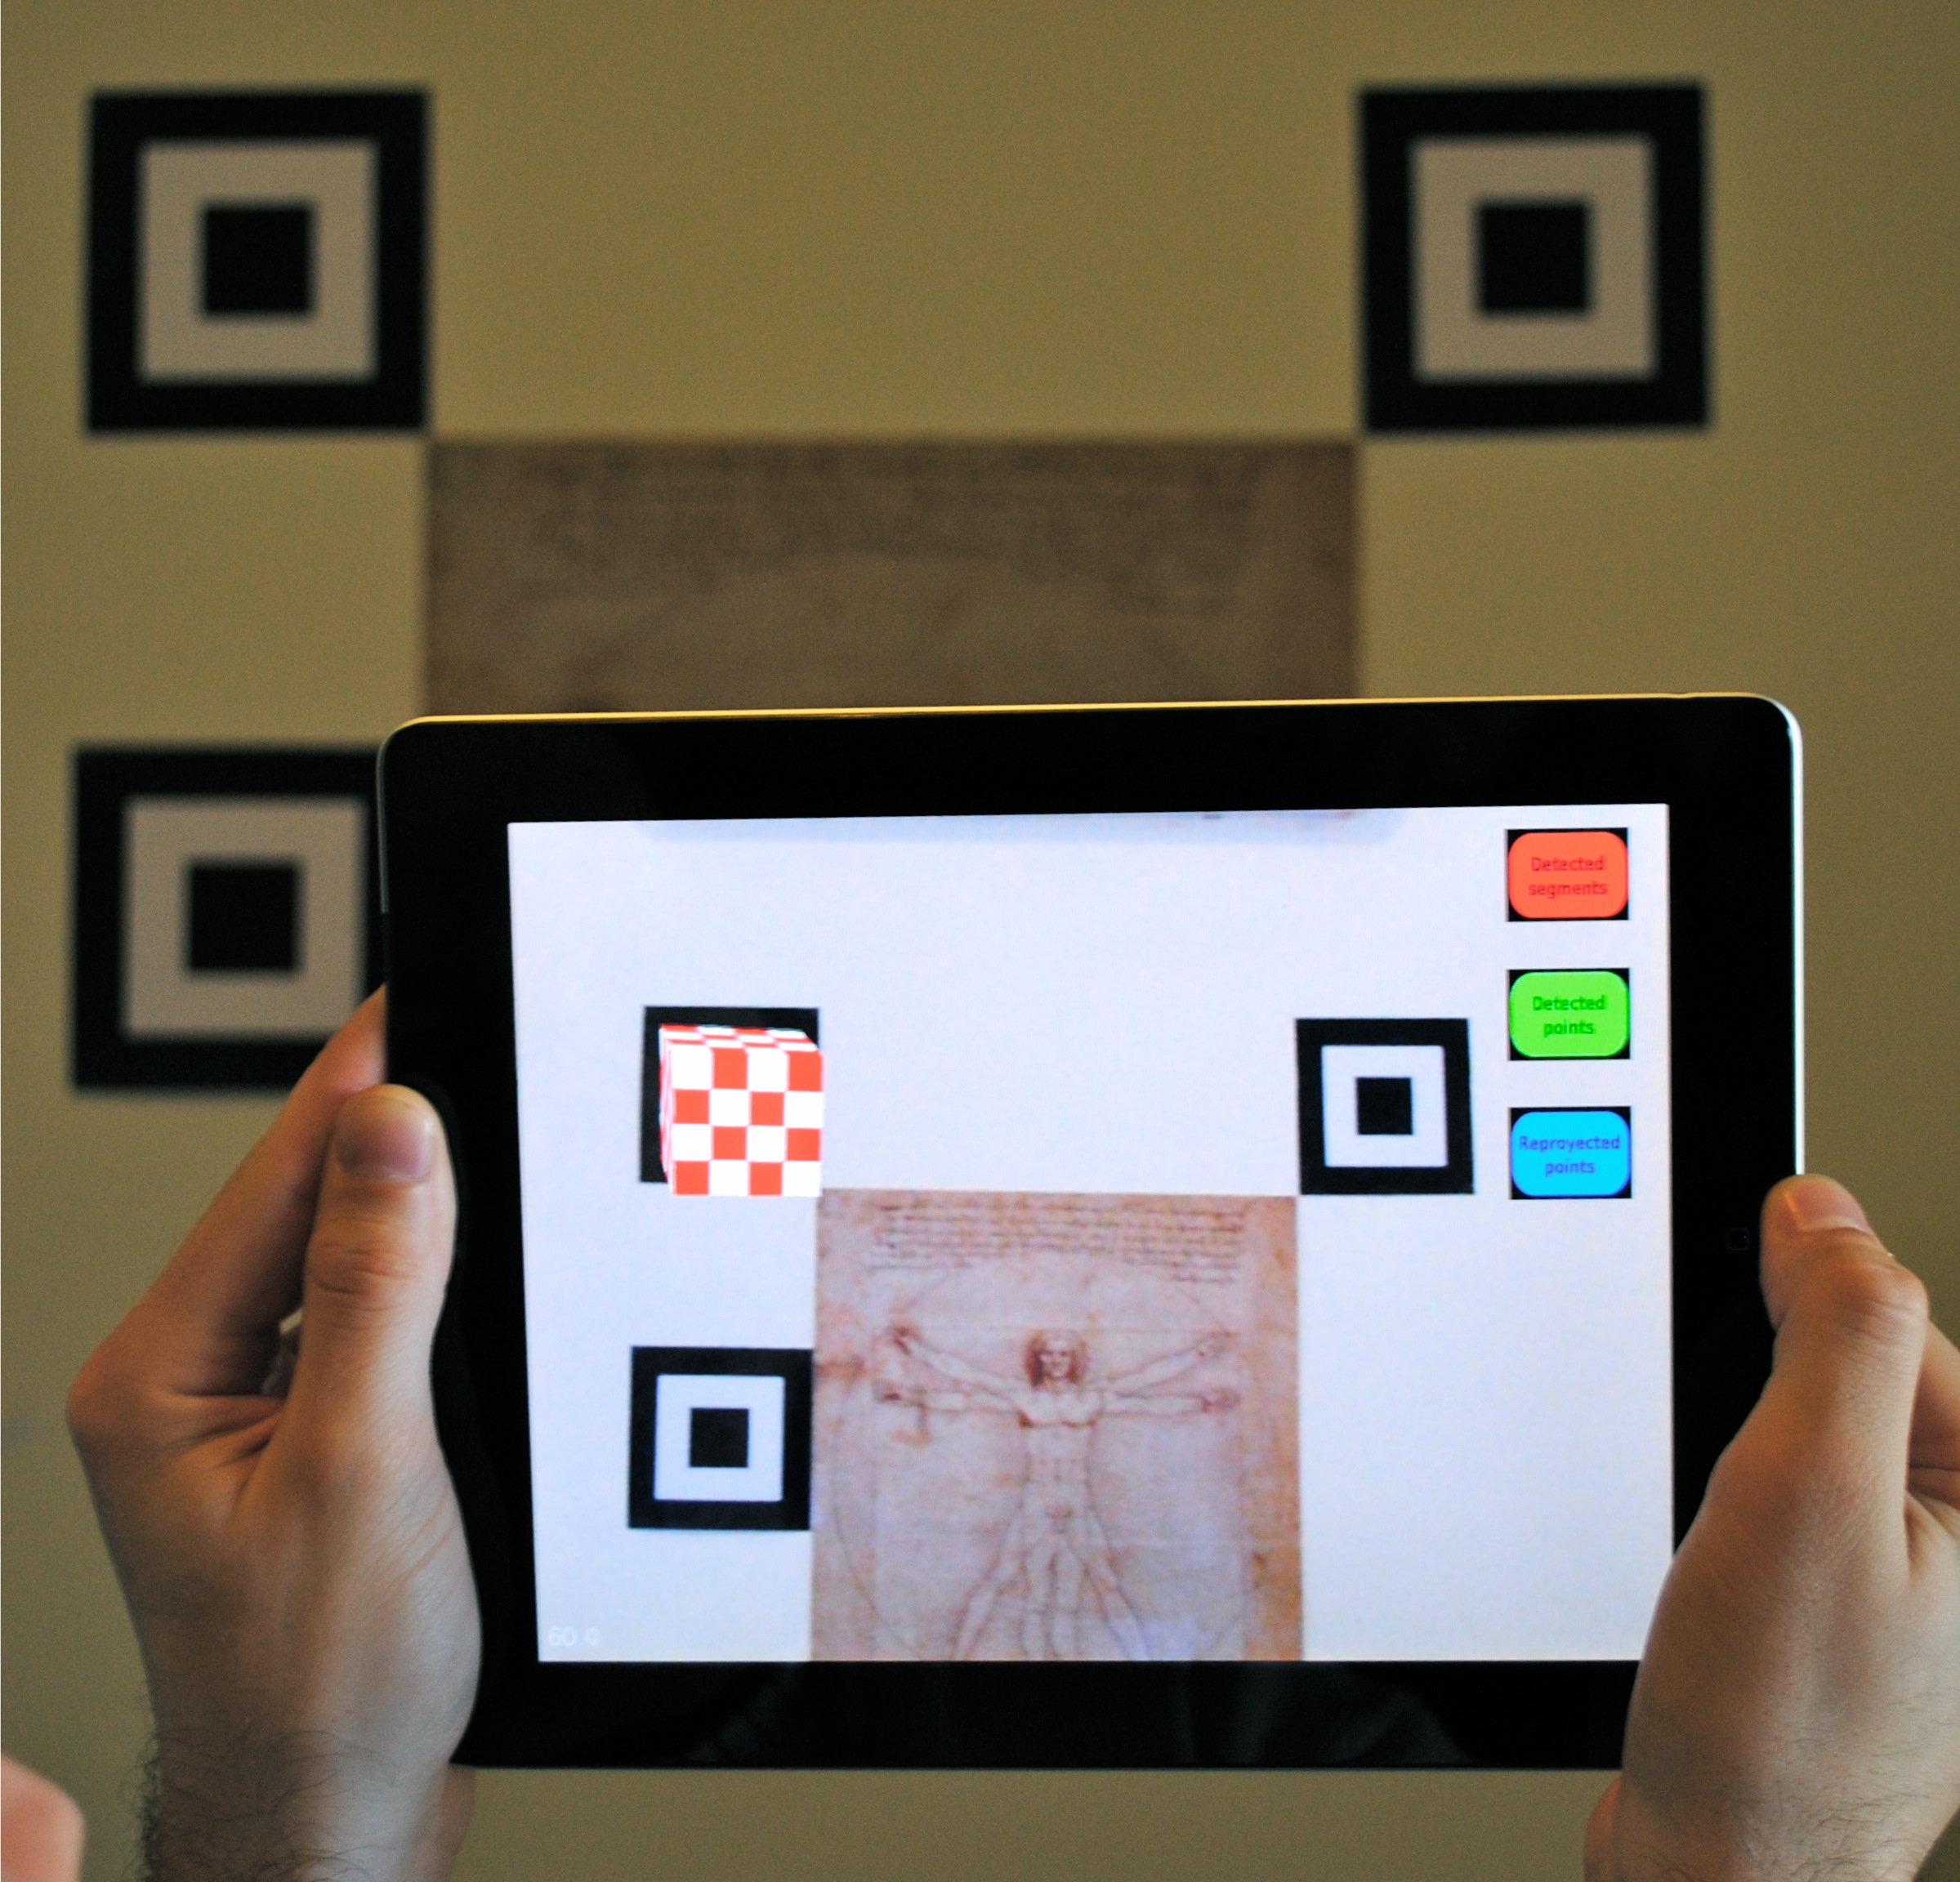
\includegraphics[scale=0.1]{figs_intro/arIntro.png}
	\label{fig: arIntro}
         \caption{Ejemplo de realidad aumentada. En la figura se puede ver c�mo se ubica un cubo virtual en la esquina superior izquierda de una r�plica de la obra ``Hombre de Vitruvio'' de Leonardo da Vinci.}
\end{figure}